\documentclass{amsproc}
\usepackage{master}
\begin{document}
\author{Lectures: Peter Ozsv\'ath and Zolt\'an Sz\'abo \\
Notes: Jackson Van Dyke}
\thanks{All errors introduced are my own.}
\date{June 11-15th, 2018}
\title{Bordered knot invariants}
\maketitle
\tableofcontents

\section{Classical knot theory}

\subsection{Preliminaries}

A knot can be regarded either as an embedding $K\inj S^3$
or $K\inj \RR^3$.
We will deal only with piecewise linear such embeddings.

\begin{exm}
We consider the preliminary example of the right-handed trefoil seen in \cref{fig:right_trefoil}
\begin{figure}
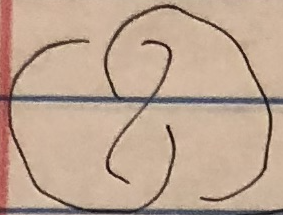
\includegraphics[width=0.5\textwidth]{trefoil_right.png}
\caption{Right-handed trefoil knot.}
\label{fig:right_trefoil}
\end{figure}
\end{exm}

We are just interested in such things modulo isotopy, so such a picture 
does indeed specify a knot.

There is a particular type of knot called a \emph{torus knot},
which lies on the surface of an unknotted torus in $\RR^3$. 
This is characterized by two integers $p,q\in \ZZ$ such that\footnote{
If we do not have this relatively prime condition, then this is a \emph{Torus link}
with more than one component.} $\left( p,q \right) = 1$.
In particular, it wraps $p$ times around
its axis of rotational symmetry and $q$ times around the interior of the torus as in 
\cref{fig:torus_knot}.
Note that the torus knot is trivial iff either $p$ or $q$ is $\pm 1$.
If we consider the intersection of the solution sets of the following:
\begin{align}
x^p + y^q = 0
&&
\abs{x} + \abs{y} = 1
\end{align}
in $\CC^2$, we get the same knot.

\begin{figure}
\centering
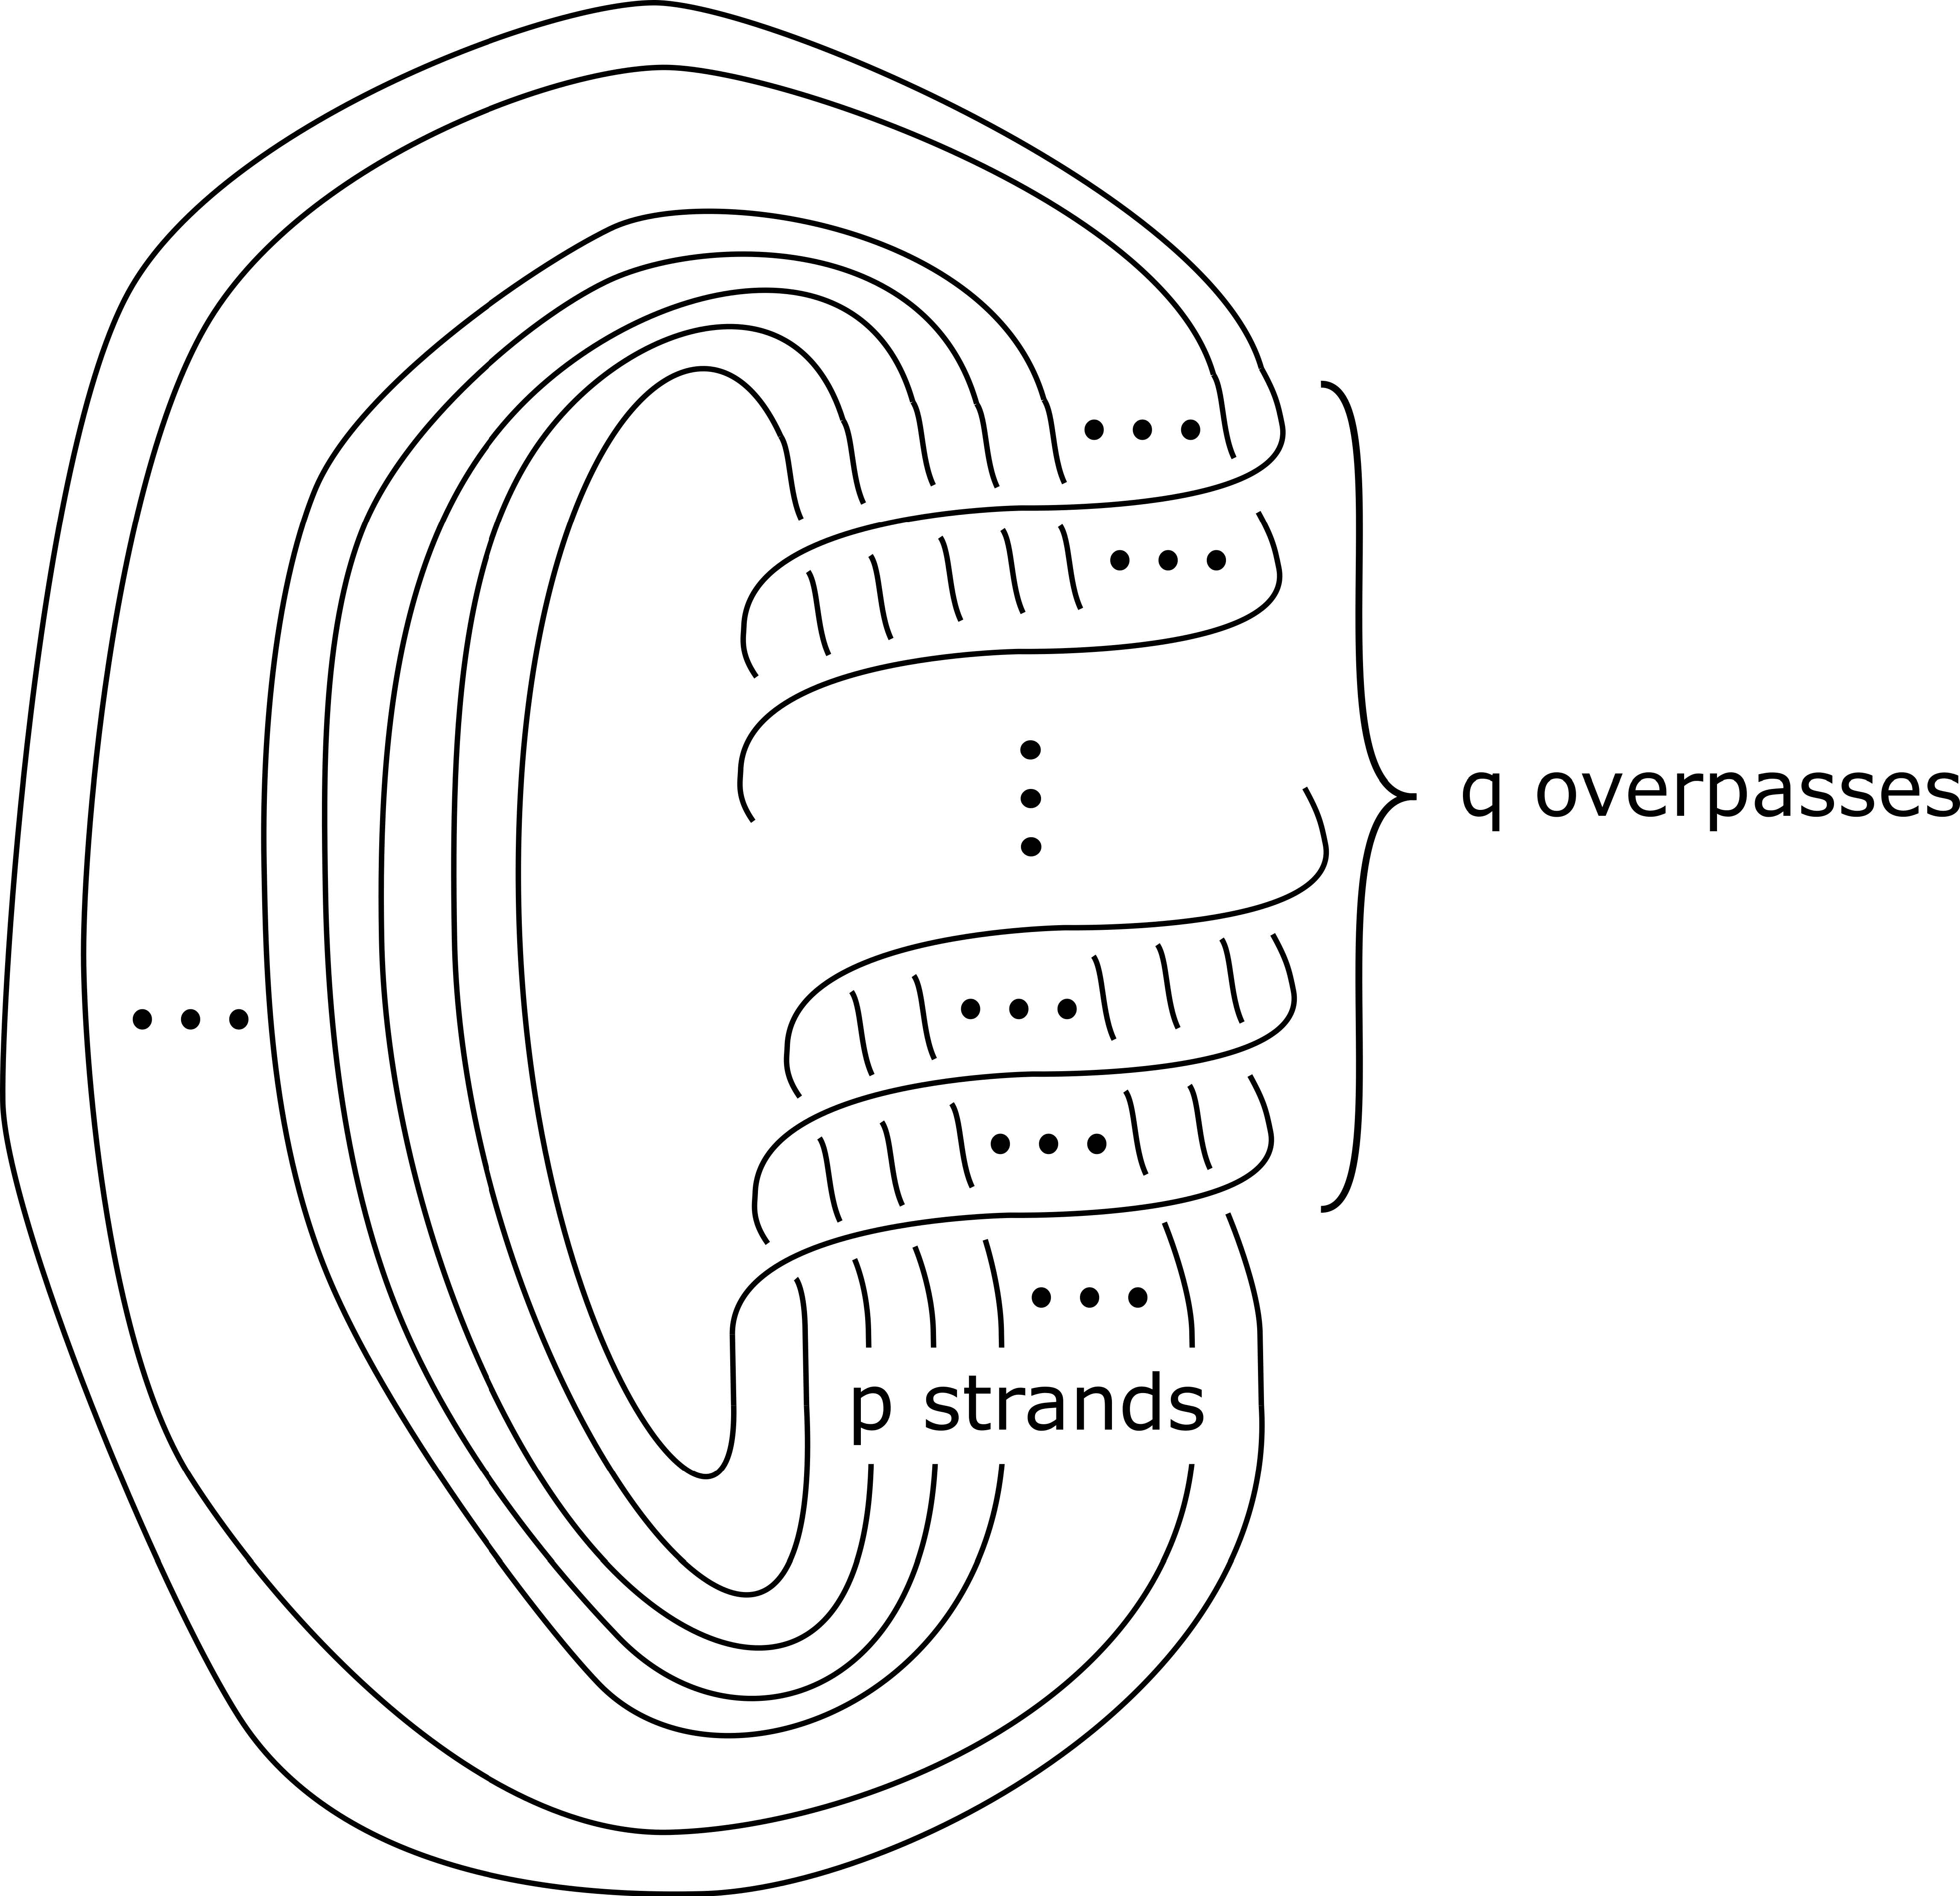
\includegraphics[width=0.5\textwidth]{torus_knot.jpg}
\caption{The $p,q$-torus knot.}
\label{fig:torus_knot}
\end{figure}

We leave the following as an exercise:

\begin{prop}
For all $p,q\in \ZZ$ such that $p,q \geq 1$ and $\left( p,q \right) = 1$, we have
$T_{p,q} = T_{q,p}$. 
\end{prop}

Another type of knot is the \emph{Pretzel knot}.
This is characterized by three integers, where these 
give the signed number of twists as in \cref{fig:pretzel_knot}.

\begin{figure}
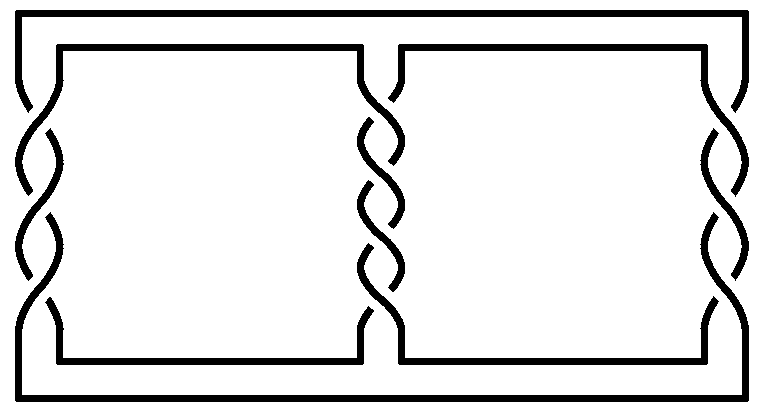
\includegraphics[width=0.5\textwidth]{pretzel.pdf}
\caption{The pretzel knot $P\left( 3 , -4 , -3 \right)$.}
\label{fig:pretzel_knot}
\end{figure}

We can also consider an \emph{oriented link} by giving each component an orientation.
Given any knot, we can reverse all crossings by switching unders and overs.
This gives us the mirror knot.

\begin{exm}
Taking the mirror of the right-handed trefoil knot gives us the 
left-handed trefoil knot as in \cref{fig:left_trefoil}.
\begin{figure}
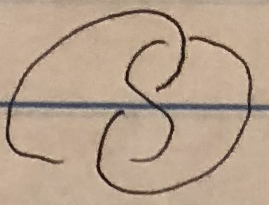
\includegraphics[width=0.5\textwidth]{trefoil_left.png}
\caption{The left trefoil knot.}
\label{fig:left_trefoil}
\end{figure}
\end{exm}

An \emph{alternating projection} of a knot is a projection such that if you follow
the knot, the crossings alternate over and under.
An \emph{alternating knot} is a knot which admits an alternating projection.

\begin{exm}
The trefoil knots we saw above are both alternating knots.
In fact, the trefoil knot is a torus knot, 
the pretzel knot $P\left( -1 ,-1, -1 \right)$, 
and an alternating knot. 
\end{exm}

\begin{rmk}
Alternating knots are somehow very well-behaved.
\end{rmk}

\begin{exr}
Which pretzel knots are torus knots?
Which pretzel knots are alternating knots?
\end{exr}

\subsection{Recognizing the unknot}

We might wonder what aspect of a knot can detect if the knot is itself the unknot. 
In order to consider this, we introduce the concept of a Redemeister move.
These can be seen in \cref{fig:redemeister}.

\begin{figure}
\centering
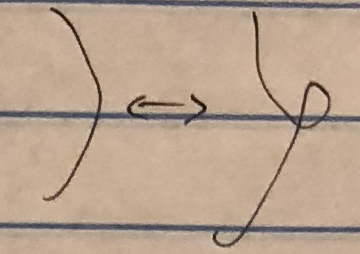
\includegraphics[width=0.5\textwidth]{r1.png}
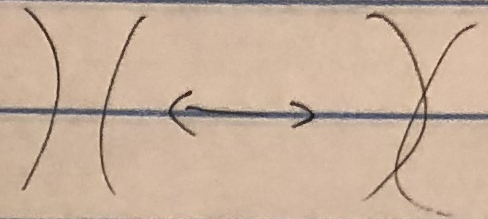
\includegraphics[width=0.5\textwidth]{r2.png}\\
\begin{tikzpicture}[knot gap = 7,baseline]
\draw[thick,knot=black](2,-0.5) -- (0,-1.5);
\draw[thick,knot=black](1,1.5) -- (1,-1.5);
\draw[thick,knot=black](0,1.5) -- (2,-1.5);
\end{tikzpicture}
$\qquad\qquad=\qquad\qquad$
\begin{tikzpicture}[knot gap = 7,baseline]
\draw[thick,knot=black](2,1.5) -- (0,0.5);
\draw[thick,knot=black](1,1.5) -- (1,-1.5);
\draw[thick,knot=black](0,1.5) -- (2,-1.5);
\end{tikzpicture}
\caption{The Redemeister moves $R1$, $R2$, and $R3$.}
\label{fig:redemeister}
\end{figure}

\begin{thm}
If two projections represent the same knot, then one can be obtained from the other
using the Redemeister moves.
\end{thm}

Knot Floer homology is an invariant of a knot. 
This is the categorification of the Alexander polynomial which we will meet later. 
There is also Khovanov homology which is the categorification of the Jones polynomial.

\begin{con}
If $K$ is a nontrivial knot, then the corresponding Jones polynomial is nontrivial.
\end{con}

\begin{thm}
Khovanov homology recognizes the unknot.
\end{thm}

\begin{thm}
Knot Floer homology recognizes the unknot.
\end{thm}

\begin{thm}
The fundamental group of the complement of a knot $K$ recognizes when it is the unknot.
\end{thm}

\begin{wrn}
Typically in our analysis of a knot, we consider a projection of the knot and 
analyse it this way. We have to be a bit careful sometimes, because if we are studying invariants, 
we need to assure that we are actually studying invariants of the knot rather than
invariants of the particular projection.
\end{wrn}


Consider some nontrivial knot, then how many reversals of intersections are needed
to obtain the unknot?
This is easy to calculate for the simple examples we've seen.
The \emph{unknotting number} of a knot is the smallest number of reversals of crossings
which will yield the unknot.

\begin{exm}
The unknotting number of the trefoil is $1$.
\end{exm}

\begin{exr}
Show that the unknotting number of $T_{p,q}$ is bounded below by
$\left( p-1 \right)\left( q-1 \right) / 2$.
\end{exr}

In fact this unknotting number is equal to $\left( p-1 \right)\left( q-1 \right) / 2$.
The proof uses $4$-manifold invariants.

\subsection{Dehn surgery}

Consider some knot $K\inj S^3$. 
Now take $S^3 \minus \nd\left( K \right)$ and 
glue the following:
\begin{equation}
S^3\minus \nd\left( K \right)\un_\phi \left( S^1\times D^2 \right)
\end{equation}
for $\phi\in \SL\left( 2,\ZZ \right)$ determined by two integers
giving a winding number through the hole of the torus, 
and one around the axis of rotational symmetry.
Now since we have $T^2 = \p\left( S^3\minus \nd\left( K \right) \right)$ we have
\begin{equation}
i:T^2 \fromto S^3\minus \nd\left( K \right)
\end{equation}
The first homologies here are $\ZZ \dsum \ZZ$ and $\ZZ$.
This whole operation is called $p / q$ surgery, and yields
$S^3_{p / q}\left( K \right)$ which has first homology $\ZZ / p \ZZ$.
Note that $1 / n$ surgery yields the homology $3$-sphere.

\begin{thm}
As long as $K$ is not the unknot, for any $r = p / q\in \QQ$, 
$S^3_{p / q}\left( K \right) \neq S_{p/q}^3 \left( U \right)$
where $U$ is the unknot.
\end{thm}

\section{Kauffman states}

For a given projection of a knot, we have $n$ crossings, 
and $n+2$ regions. 
Now we choose a marked edge, and decide that the adjacent regions
are special, leaving us with $n$ crossings and $n$ regions. 
Now a \emph{Kauffman corner} is a choice of a crossing, and a region.

\begin{defn}
Let $K$ be a knot with a projection having $n$ crossings. 
Then a \emph{Kauffman state} is a choice of $n$ corners:
$S = \left\{ c_1 , \cdots , c_n \right\}$ such that each region gets exactly $1$ corner, 
except the marked regions, and each crossing gets exactly $1$ corner.
\end{defn}

We always have a finite amount, and for a knot we always have an odd number.

\subsection{Black and white graphs}

The \emph{black graph} (resp. \emph{white graph})
is constructed as follows.
Color each region of the projection of some knot either black and white such that
no adjacent pair of regions share a color.\footnote{
We can see that this is always possible by drawing an arc from any region
out to infinity, and then counting the number of edges it crossed. 
We then assign a color to the region according to parity.}
Then the vertices of the graph are given by the black (resp. white) regions, 
and the edges are given by the crossings.
This can be pictured in \cref{fig:graph_examples}.
\begin{figure}
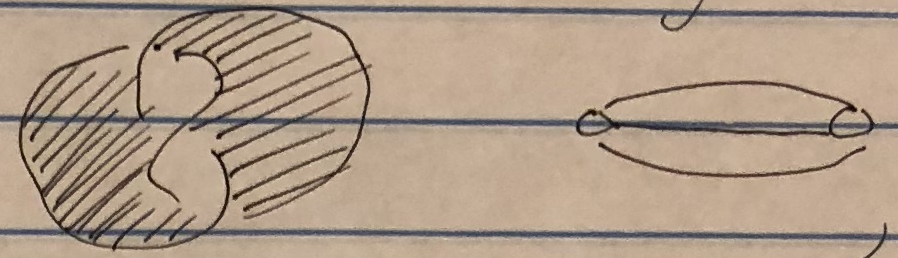
\includegraphics[width=0.5\textwidth]{trefoil_graph.png}
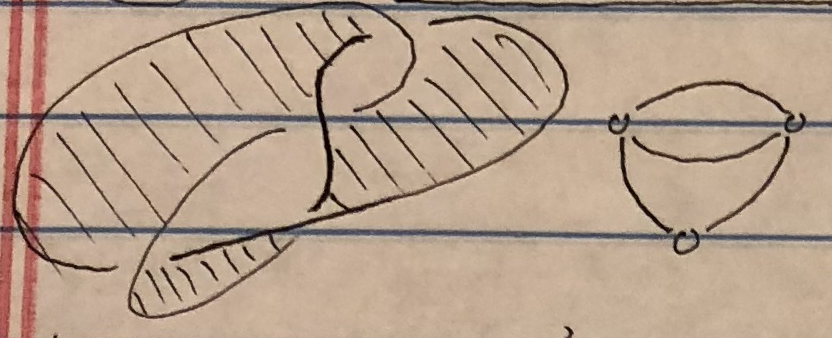
\includegraphics[width=0.5\textwidth]{figure_eight_graph.png}
\caption{The black graphs for the figure eight knot and right-handed
trefoil.}
\label{fig:graph_examples}
\end{figure}

Now we define some conventions to assign certain numbers to crossings.
We can see these choices in \cref{fig:pos_neg_crossings}.
As it turns out, the full contribution of these gradings for a given state is always an integer.
This is clearly true for the Maslov grading, but is also true for the Alexander grading.
\begin{figure}
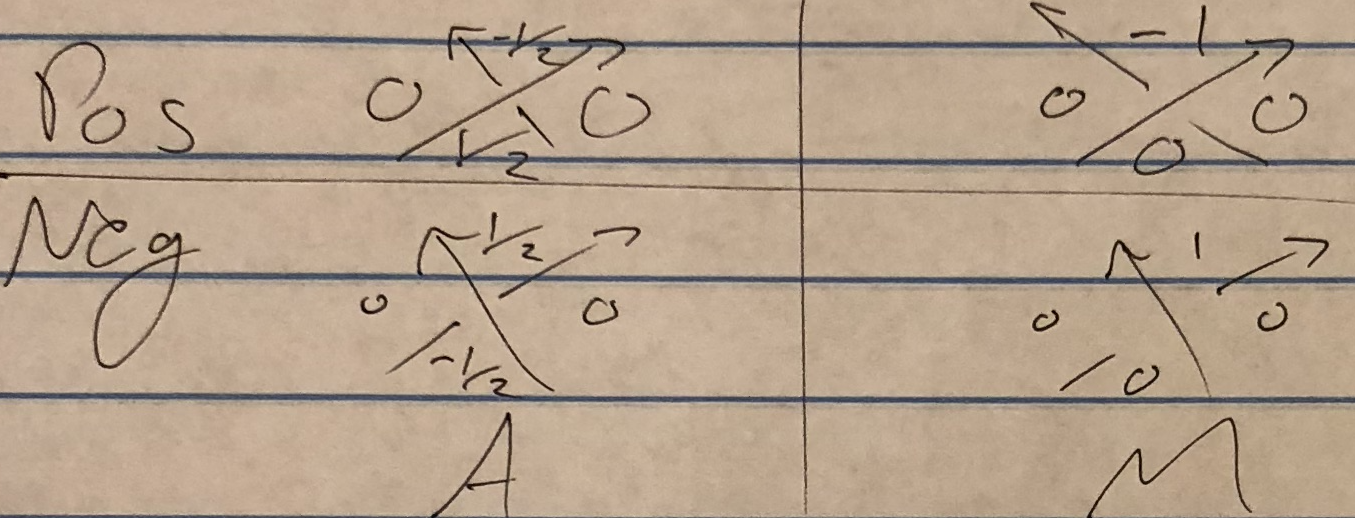
\includegraphics[width=0.5\textwidth]{gradings.png}
\caption{On the top we have the right-handed or positive crossing and the
associated Maslov grading $M$, and Alexander grading $A$. 
On the bottom we have the same for the left-handed or negative crossing.}
\label{fig:pos_neg_crossings}
\end{figure}
Now to every corner $c$ we will associate the term 
$t^{A\left( c \right)} \left( -1 \right)^{M\left( C \right)}$, so we get 
\begin{equation}
S = \left( c_1 , \cdots , c_n \right)
\fromto
\prod_{i = 1}^n t^{A\left( c_i \right)} \left( -1 \right)^{M\left( c_i \right)}
\end{equation}

\subsection{The Alexander polynomial}

Now to get the actual Alexander polynomial we take the following sum:
\begin{equation}
A\left( D , e \right) = 
\sum_{S\in \text{Kauffman states}}
\left( -1 \right)^{M\left( S \right)} t^{A\left( S \right)} 
\end{equation}

\begin{exm}
Consider the unknot drawn as in \cref{fig:unknot_twisted}
\todo{figure}
\begin{figure}
\caption{The unknot with a twist, as to allow for a nonempty set of
Kauffman states.}
\label{fig:unknot_twisted}
\end{figure}
This makes it clear that the Alexander polynomial is just $1$.
\end{exm}

\begin{exm}
Consider the trefoil knot. This has three different Kauffman states illustrated in
\cref{fig:trefoil_kauffman}.
\begin{figure}
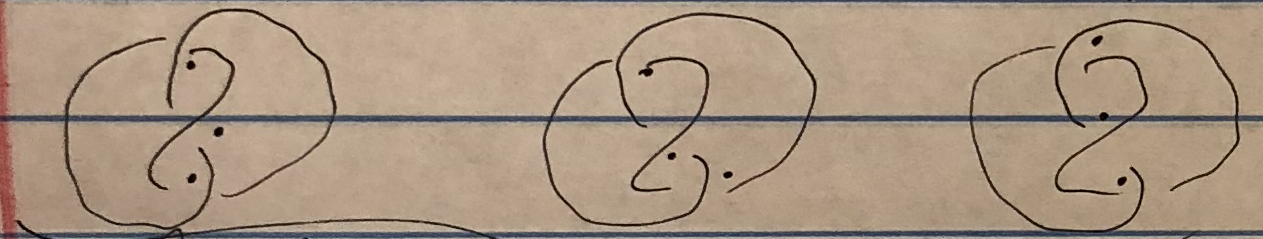
\includegraphics[width=0.7\textwidth]{trefoil_kauffmann_states.png}
\caption{The three Kauffman states for the trefoil knot.}
\label{fig:trefoil_kauffman}
\end{figure}
The contributions of these states in terms of gradings are plotted in 
\cref{fig:trefoil_gradings}
\begin{figure}
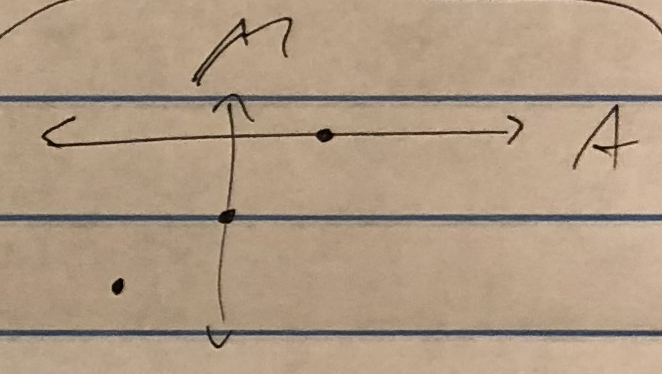
\includegraphics[width=0.5\textwidth]{gradings_trefoil_kauffmann_states.png}
\caption{The plotted gradings are plotted for the three Kauffman states of
the trefoil knot.}
\label{fig:trefoil_gradings}
\end{figure}
All together the Alexander polynomial is:
\begin{equation}
t - 1 + \frac{1}{t}
\end{equation}
\end{exm}

\begin{thm}
The Alexander polynomial is an invariant for any knot $K$. 
\end{thm}

\begin{proof}
We have to show that it is invariant under the Redemeister moves, and is independent of 
the marked edge. 
We leave it as an exercise to show that the contributions on both sides of the Redemeister moves
cancel.
To see it is independent of the marked edge, we consider a corner locally, and pull the edge
down and around $S^3$ until it comes back up the other side, so we can effectively move the marking
over crossings. 
\end{proof}

\begin{thm}
\begin{equation}
A_{K_+} - A_{K_-} = A_{K_0} \left( t^{1/2} - t^{-1/2} \right)
\end{equation}
\end{thm}


\section{Heegaard Floer homology}

\subsection{Heegaard diagrams}

Consider a surface $\Sigma_g$ of genus $g$. 
A \emph{complete set of attaching circles} for $\Sigma_g$
is a collection of $g$ pairwise disjoint, homologically linearly independent simple,
closed curves. 
Such a collection of circles specifies some handlebody $U_\gamma$ which has
$\Sigma_g$ as its boundary. That is, the attaching circles bound disjoint embedded disks in $U_\gamma$.

Now suppose $Y$ is a closed, oriented $3$-dimensional manifold. 
Then a \emph{Heegaard splitting} of $Y$ is a decomposition of $Y$ as the union of two handlebodies
glued along their boundary. 

\begin{exm}
The simplest example is cutting $S^3$ into two balls of genus $0$.
We could alternatively cut out a tubular neighborhood of the unknot to get
a Heegaard decomposition of genus $1$.
\end{exm}

We can encode the information of a Heegaard splitting as combinatorial data using  
a \emph{Heegaard diagram} $\cH = \left( \Sigma, \vec{\al} , \vec{\b} \right)$, where
\begin{align}
\vec{\al} = \left\{ \al_1 , \cdots , \al_g \right\}
&&
\vec{\b} = \left\{ \b_1 , \cdots , \b_g \right\}
\end{align}
are two complete sets of attaching circles for $\Sigma$.
We will typically consider pointed Heegaard diagrams, where we take a marked point $w$
disjoint from the $\al_i$ and $\b_i$.
We can also consider the Heegaard diagram of $Y$ from a slightly different point of view.
Equip $Y$ with a self-indexing Morse function $f$ and gradient-like vector field $v$. 
Then $\Sigma$ can be taken to be $f^{-1}\left( 3/2 \right)$, 
$\vec{\al}$ can be taken to be the locus of points 
that flow out of the index one critical points under $c$,
and $\vec{\b}$ can be taken to be the locus of points that flow into the index two 
critical points.

From the attaching circles we can form the tori:
\begin{align}
\TT_\al = \al_1 \times \cdots \times \al_g
&&
\TT_\b = \b_1 \times \cdots \times \b_g
\end{align}
Said more concretely, $\TT_\al$ (resp. $\TT_\b$) consists of
$g$-tuples in $\Sigma_g$, where each point is on some $\al_i$ (resp. $\b_i$) 
no two points lie on the same $\al_i$ (resp. $\b_i$).
Recall the $d$-fold symmetric product is defined as:
\begin{equation}
\Sym^d\left( \Sigma \right) = \frac{\obr{\Sigma \times \cdots \times \Sigma}{d}}{S_d}
\end{equation}
Now define the subspace $V_w\sub \Sym^g\left( \Sigma \right)$ 
to consist of the $g$-tuples in $\Sym^g\left( \Sigma \right)$
which include the marked point $w$.
Then the intersection points $\TT_\al$ and $\TT_\b$ are the \emph{Heegaard states}
$\cS\left( \cH \right)$.
Explicitly, Heegaard states of type $\sigma$ correspond to points in the product:
\begin{equation}
\left( \al_1 \cap \b_{\sigma\left( 1 \right)} \right) \times \cdots \times
\left( \al_g \cap \b_{\sigma\left( g \right)} \right)
\end{equation}
A complex structure on $\Sigma$ naturally induces a complex structure on the $g$-fold
symmetric product $\Sym^g\left( \Sigma \right)$. 
We can even give this a K\"ahler structure so $\TT_\al$ and $\TT_\b$ are Lagrangian, 
and now variants of the Heegaard Floer homology of $Y$ correspond to variants of the
Lagrangian Floer homology of $\TT_\al$ and $\TT_\b$ in $\Sym^g\left( \Sigma \right)$.
See \cite{auroux_fukaya} for an approachable introduction to Lagrangian Floer homology.

A given surface might have many different Heegaard diagrams, so how do we
know when two diagrams correspond to the same surface?
We have the following Heegaard moves:
\begin{figure}
\centering
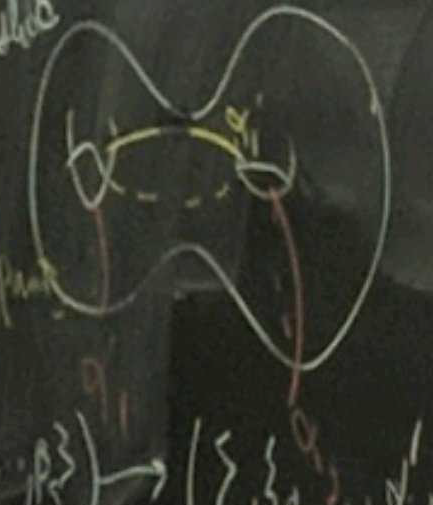
\includegraphics[width=0.4\textwidth]{handle_slide.png}
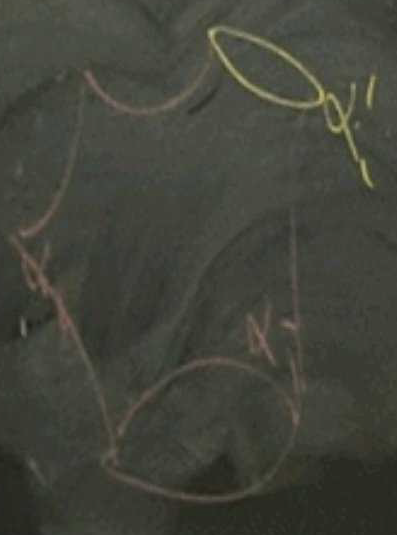
\includegraphics[width=0.4\textwidth]{pants.png}
\caption{Handle sliding $\al_1$ over $\al_2$.}
\label{fig:handle_slide}
\end{figure}
\begin{enumerate}
\item Isotope $\al_i$ or $\b_i$
\item Handle slide: Given that some $\al_i' , \al_i , \al_j$ 
bound a pair of pants in $\Sigma$ disjoint from all
other $\al_k$, then we replace $\al_i$ with $\al_i'$.
This can be visualized in \cref{fig:handle_slide}.

\item Stabilization: 
Given $\Sigma , \left\{ \al_i \right\}, \left\{ \b_i \right\}$, 
we can always just take
\begin{equation}
\left( \Sigma \# T^2,
\left\{ \al_1 , \cdots , \al_g , \al_{g+1} \right\} , 
\left\{ \b_1 , \cdots , \b_g , \b_{g+1} \right\}\right)
\end{equation}
This corresponds to adding extra handles as in \cref{fig:stabilization}.
\begin{figure}
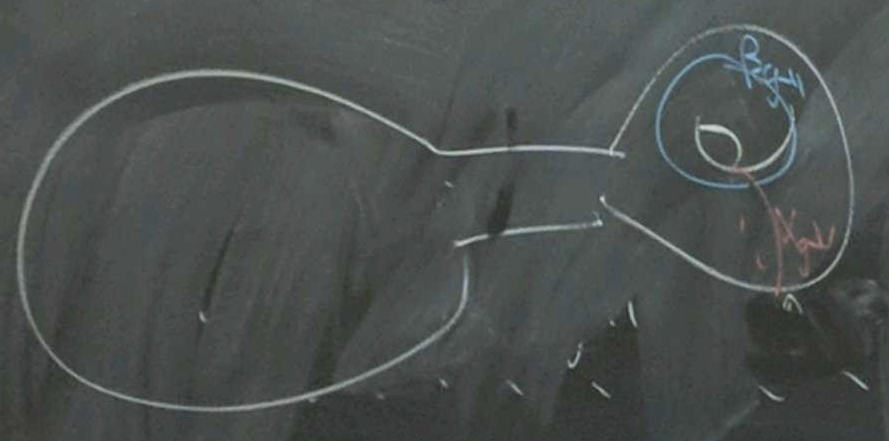
\includegraphics[width=0.5\textwidth]{stabilization.png}
\caption{Visualizing the Heegaard stabilization move as adding
an extra handle.}
\label{fig:stabilization}
\end{figure}
\end{enumerate}

\begin{thm}
Any two Heegaard diagrams which are equivalent 
under these three moves represent the same surface.
\end{thm}

\begin{exm}
The genus $1$ Heegaard decomposition of $S^3$ from above gives us a diagram
$\left( \Sigma_1 , \left\{ \al_1 \right\} , \left\{ \b_1 \right\} \right)$, 
where $\al_1$ and $\b_1$ meet transversely
at a unique point.
Note that $S^1\times S^2$ corresponds to 
$\left( \Sigma_1 , \left\{ \al_1 \right\} , \left\{ \al_1 \right\}\right)$.
\end{exm}

\begin{exm}
The lens space $L\left( p,q \right)$ has a Heegaard diagram
$\left( \Sigma_1 , \al , \b \right)$ where $\al$ and $\b$ intersect at $p$ points.
\end{exm}


\subsection{The chain complex}

Equip $\Sym^g\left( \Sigma \right)$ with compatible almost complex
and symplectic structures.
For two Heegaard states $x$ and 4y, we can consider the pseudo-holomorphic
disks in $\Sym^g\left( \Sigma \right)$, and in particular we can organize these into
homotopy classes of maps $u:\DD\fromto \Sym^g\left( \Sigma \right)$ mapping the unit
disk into $\Sym^g\left( \Sigma \right)$, which map $-i$ to $x$, $i$ to $y$,
and for all $z = x + iy \in \p \DD$,
\begin{equation}
u\left( x+ iy \right) \in
\begin{cases}
\TT_\al & x \geq 0 \\
\TT_\b & x\leq 0
\end{cases}
\end{equation}
We write $\pi_2\left( x , y \right)$ for these homotopy classes.

Denote the Grassmannian of Lagrangian $n$-planes in
$\left( \RR^{2n} , \om_\std \right)$ by $\LGr\left( n \right)$.
It is well known that $\U\left( n \right)$ acts transitively on $\LGr\left( n \right)$, 
which means $\LGr\left( n \right) \simeq \U\left( n \right) / \O\left( n \right)$.
From this it follows that $\pi_1\left( \LGr\left( n \right) \right) \simeq \ZZ$.
Explicitly we can take the square of the determinant to get
a map $\U\left( n \right) / \O\left( n \right) \fromto S^1$
which induces an isomorphism on the fundamental groups.
Then we define the \emph{Maslov index} of a loop in $\LGr\left( n \right)$ to
be the winding number of its image under this map.

Now we define the map $n_w : \pi_2\left( x , y \right) \fromto \ZZ$, 
by taking the algebraic intersection number of a generic
$u$ representing a class $\phi \in \pi_2\left( x , y \right)$ with $V_w$. 
Note that this is well-defined since we took $w$ to be disjoint 
from the $\al_i$ and $\b_i$. 
The moduli-space of pseudo-holomorphic disks representing $\phi$ will be written
$\cM\left( \phi \right)$. 
This has a natural $\RR$ action given by automorphisms of $\DD$ preserving $\pm i$.

Take $\hatt{\CF}$ to be the vector space generated by $\cS\left( \cH \right)$ over
$\FF$ equipped with the differential:
\begin{equation}
\hatt{\p}\left( x \right) = 
\sum_{y\in \cS}
\sum_{\left\{ \phi \in \pi_2\left( x, y \right) \st 
n_w\left( \phi \right)= 0, \mu\left( \phi \right) = 1 \right\}}
\#\left( \frac{\cM\left( \phi \right)}{\RR} \right)y
\end{equation}
where $\mu\left( \phi \right)$ is the Maslov index.
There is a refinement of this theory, where we take $\CF^-\left( \cH \right)$ 
to instead be a module over the polynomial algebra $\FF\left[ U \right]$,
and define the differential to be:
\begin{equation}
\p^-\left( x \right)= \sum_{y\in \cS} \sum_{
\left\{ \phi \in \pi_2\left( x , y \right) \st \mu\left( \phi \right)= 1 \right\}}
\#\left( \frac{\cM\left( \phi \right)}{\RR} \right) U^{n_w\left( \phi \right)} y
\end{equation}
As it turns out, by the main theorem of \cite{oz_sz_three_manifolds}
these are both invariants of the underlying closed, oriented three-manifold $Y$, 
represented by $\cH$.



\section{Knot Floer homology}

The so-called knot Floer homology, 
is a slight extension of the Heegaard Floer homology
developed in the previous section.

\subsection{Getting a knot projection from a Heegaard diagram and vice versa}

Consider a knot $K\inj Y$ embedded in a $3$-manifold. 
Suppose we have a Heegaard diagram $\left( \Sigma , \vec{\al} , \vec{\b} , w , z \right)$
with two base-points. We specify the knot as follows. 
Connect $w$ and $z$ in $\Sigma$ by an arc which is disjoint from all of the $\al_i$. 
Then connect $w$ and $z$ in $\Sigma$ by an arc which is disjoint from all of the $\b_i$, 
and connect the arcs. This can be oriented by taking $\p a = z - w = - \p b$.

We now go in the opposite direction. Consider a knot $K\inj Y$. Take some decorated projection of the knot,
so we have some marked edge, 
and singularize\footnote{This just means we forget the crossings.} the projection.
Now take a regular neighborhood of the resulting graph to get a handlebody.
That is we just sort of thicken the knot without concerning ourselves over the crossings. 
Now the marked edge of the projection gives us two distinguished regions in the 
complement of the projection, one of which is the infinite region.
For each of the bounded regions, we associate an $\al$ circle, and to each
crossing, we associate a $\b$ circle. We choose a final $\b$ circle transverse to the 
marking on the distinguished edge. Now place basepoints $w$ and $z$ on either side of this
final $\b$-circle.
An example of this whole construction can be seen in \cref{fig:doubly_pointed}.

\begin{figure}
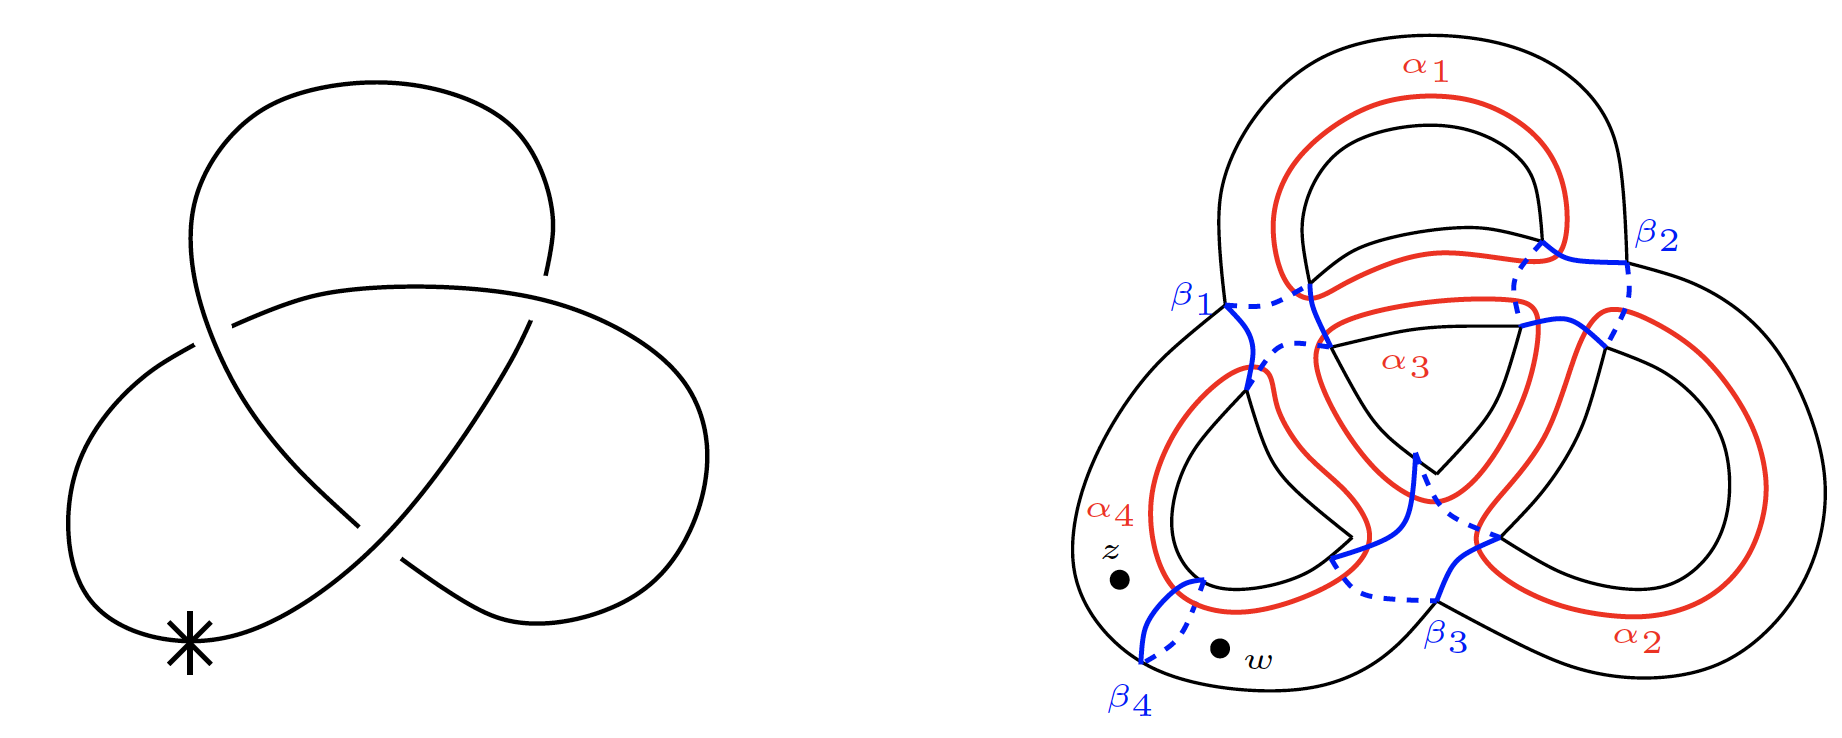
\includegraphics[width=0.5\textwidth]{doubly_pointed.png}
\caption{Doubly-pointed Heegaard diagram for the left-
handed trefoil knot.}
\label{fig:doubly_pointed}
\end{figure}

It is not obvious that we will always get $g$ $\al$ and $\b$-circles.
To see this, first notice that the planar graph resulting from singularizing the knot projection
is certainly connected, so it has Euler characteristic
$\chi\left( K \right) = 2 = V - E + F$, where $V$ is the number of crossings, 
$F$ is the number of connected components, and $E$ is the number of edges. 
We also know $E = 2V$ for this graph, so $2 = F - V$. By construction, we have that the genus of the
surface will be $g = F - 1$, and the number of $\al$ curves will also be $g = F-1$, so we have
$2 = g + 1 - V$, so we have $V = g - 1$ crossings, and therefore $g - 1$ $\b$-circles, so along with
the additional one we added, we get $g$ in total.

\subsection{The chain complex of a $3$-manifold}

Now that we know how to associate a Heegaard diagram with every knot, we can form
the chain complex $\hatt{\CFK}\left( \cH \right)$ generated by the Heegaard states
over $\FF$. The differential is given by:

\begin{equation}
\hatt{\p}_K\left( x \right) = 
\sum_{y\in \cS} \sum_{ \left\{ \phi \in \pi_2\left( x , y \right) \st
n_w\left( \phi \right) = 0 = n_z\left( \phi \right), \mu\left( \phi \right) =1\right\}}
\#\left( \frac{\cM\left( \phi \right)}{\RR} \right) y
\end{equation}


\subsection{Grading}

We will equip this complex with a bigrading. 
That is, we want functions $M$ and $A$
which map $\cS\left( \cH \right) \fromto \ZZ$.
These will only be defined up to an additive constant, so we will actually define 
these functions on pairs of states, and show that this is really just
the difference of the values for the individual states.

\begin{lem}
For any pair $\left( x,y \right)$ of intersection points of a Heegaard diagram of $S^3$, 
there exist some $\phi \in \pi_2\left( x , y \right)$.
\end{lem}

Define the following:
\begin{align}
A\left( x , y \right) &= n_z\left( \phi \right) - n_w\left( \phi \right)
\\
M\left( x , y \right) &= \mu\left( \phi \right) - 2 n_w\left( \phi \right)
\end{align}
where $\phi \in \pi_2\left( x , y \right)$.

\begin{fact}
These are well defined.
\end{fact}

\begin{fact}
There exists $A:\TT_\al \cap \TT_\b \fromto \ZZ$ such that
$A\left( x \right) - A\left( y \right) = A\left( x , y \right)$.
and $M : \TT_\al \cap \TT_\b \fromto \ZZ$ such that
$M\left( x \right) - M\left( y \right) = M\left( x , y \right)$.
\end{fact}

\begin{fact}
There is only one lift of this function such that the 
Euler characteristic is the Alexander polynomial.
\end{fact}

\subsection{Other variants of knot Floer homology}

We will use a filtration to build the complex $\CFK$, which
is a variant of $\hatt{\CFK}$ from above.

\begin{defn}
Suppose we have a chain complex $\left( \cC_* , \p \right)$.
A filtration is a function $\cF:\cC_*\fromto \ZZ$ such that 
$\cF\left( \p x \right)\leq \cF\left( x \right)$. 
\end{defn}

A filtration can be thought of as an increasing
sequence of subcomplexes, such that the union is the full complex.

Take the generators $c\in \CF$ with $A\left( c \right) \leq i$. 

We want to extend $A$ to chains. 
A chain is a sum of $u$ powers times generators:
\begin{equation}
c = \sum_i u^{m_i} x_i
\end{equation}
Then we have:
\begin{align}
A\left( u^{m_i} x_i \right) = A\left( x_i \right) - m_i
&&
A\left( \sum_i u^{m_i} x_i \right) = 
\max_i A\left( u^{m_i} x_i\right)
\end{align}

\begin{thm}
$A\left( \p x \right) \leq A\left( x \right)$
\end{thm}

This means
\begin{equation}
\cF_i = \left\{ c\in \CF \st A\left( c \right) \leq i \right\}
\end{equation}
is indeed a filtration.

Now define:
\begin{equation}
\CFK \ceqq
\bdsum_{x\in \TT_\al \cap \TT_\b}
\FF\left[ u,v \right] x / \left\{ uv = 0 \right\}
\end{equation}
so this is a freely generated by the intersection points over
$\FF\left[ U,V \right] / UV$. This is equipped with the following differential:
\begin{equation}
\p x = \sum_y
\sum_{\phi\in \pi_2\left( x,y \right), \mu\left( \phi\right) = 1}
\frac{\cM\left( \phi \right)}{\RR} u^{n_z\left( \phi \right)} v^{n_w\left( \phi \right)} y
\end{equation}

Note that we get the following reductions:
\begin{equation}
\gr \cF = \bdsum_{i\in \ZZ} \cF_i / \cF_{i-1}
= \hatt{\CFK}
\end{equation}
\begin{equation}
H_*\left( \bdsum_{i\in \ZZ} \cF_i / \cF_{i-1} \right) = 
\hatt{\HFK}
\end{equation}

\section{Properties of knot Floer homology}

\subsection{The Alexander polynomial}

Recall the Alexander polynomial associated to a knot $K$.
There is also something called the \emph{Poincar\'e} polynomial.
This encodes all of the information of the bigraded vector space 
$\hatt{\HFK}\left( K \right)$. For a knot $K$ we define:
\begin{equation}
P_K\left( q,t \right) = \sum_{d,s} 
\dim \hatt{\HFK}_d\left( K , s \right) q^d t^s
\end{equation}

Then we have the following theorem:

\begin{thm}
Let $K$ be an alternating knot. 
Then the knot Floer homology of $K$ is determined by its Alexander polynomial
$\Delta_K\left( t \right)$ and its signature $\sigma\left( K \right)$, by the following formula:
\begin{equation}
P_K\left( q , t \right) = q^{\sigma / 2} \Delta_K\left( qt \right)
\end{equation}
\end{thm}

\subsection{Seifert genus}

The Seifert genus is a classical knot invariant.
This is another way to measure how complicated a knot is.
First we have to introduce a Seifert surface.
We want an embedded oriented surface with the knot as the boundary as in \cref{fig:seifert_motivation}.

\begin{figure}
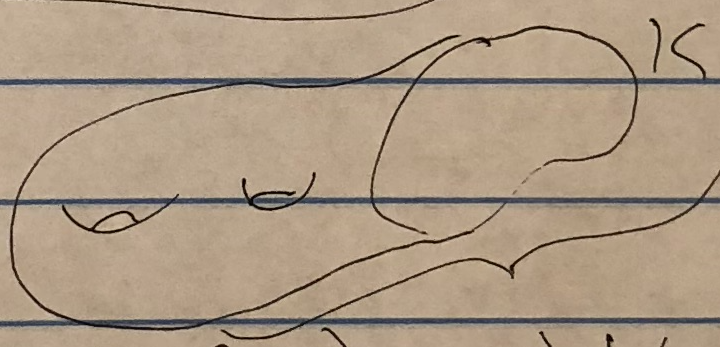
\includegraphics[width=0.5\textwidth]{seifert_surface.png}
\caption{An example of a Seifert surface for a knot $K$.}
\label{fig:seifert_motivation}
\end{figure}

\begin{exm}
The unknot clearly admits a Seifert surface, in particular the disk.
\end{exm}

\begin{exm}
The trefoil also admits a Seifert surface seen in \cref{fig:trefoil_seifert}.
\begin{figure}
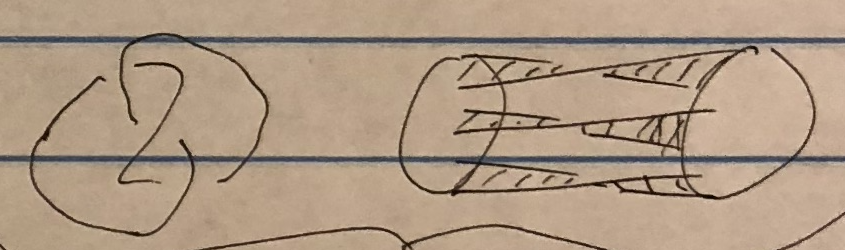
\includegraphics[width=0.5\textwidth]{trefoil_seifert.png}
\caption{The trefoil knot admits a Seifert surface
by taking two disks, and attaching one band for each crossing.}
\label{fig:trefoil_seifert}
\end{figure}
\end{exm}

In the previous example we effectively just took the black graph of the knot, and used this
to explicitly construct a Seifert surface.
For any generic knot this technique will certainly yield a surface 
with the knot as its boundary, but it won't always be oriented. 
However we actually have the following:

\begin{thm}
Every knot admits a Seifert surface. 
\end{thm}

\begin{proof}[Sketch of proof]
This is shown using Seifert's algorithm.
Loosely speaking, we take the projection, and resolve each crossing in an oriented fashion.
Now we have a union of oriented circles, which we fill with a disks, then we replace these
altered crossings with some bands.
\end{proof}

There is obviously some ambiguity in the choice of Seifert surface, and we can of course arbitrarily increase
the genus of a given Seifert surface by adding holes without altering the boundary, or the fact
that it's oriented.
Therefore we define:

\begin{defn}
The \emph{Seifert genus} is the minimal genus of a Seifert surface of a given knot. 
\end{defn}

\begin{thm}
A knot as Seifert genus $0$ iff it is the unknot.
\end{thm}

As it turns out, knot Floer homology can actually compute this Seifert genus. 
The support of $H_{*,*}\left( K \right)$ can be seen in \cref{fig:support_of_HFK}
where we write 
\begin{equation}
d = \max\left\{ i \st H_{i,*} \left( K \right) \neq 0 \right\}
\end{equation}
\begin{figure}
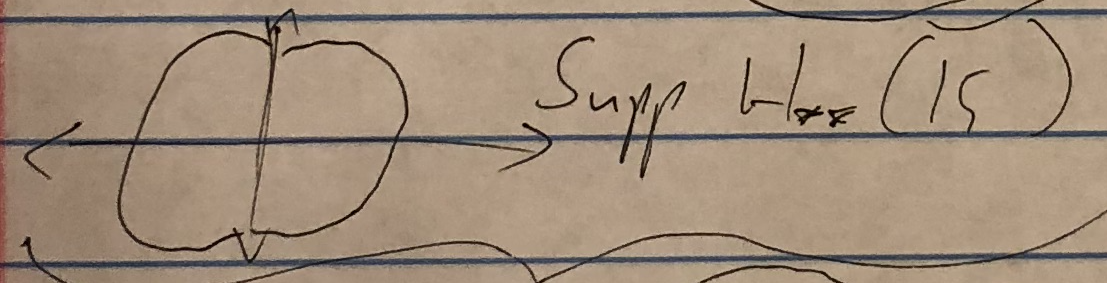
\includegraphics[width=0.5\textwidth]{homology_support.png}
\caption{The support of $H_{*,*}\left( K \right)$.}
\label{fig:support_of_HFK}
\end{figure}

\begin{thm}
$d = g\left( K \right)$
\end{thm}

\begin{cor}
If $K\neq U$, 
$H_{*,*}\left( K \right) \neq H_{*,*}\left( U \right)$
\end{cor}

\begin{thm}
A knot is fibered iff the total rank of the homology on the line at $d$ is $1$.
\end{thm}

Suppose $K$ is alternating.
Then we have seen that $\deg A_K = g\left(\Sigma \right) \geq g\left( K \right)$
for a Seifert surface $\Sigma$, 
and by one of the definitions of $A_K$, $\deg A_K \leq g\left( K \right)$.
We have the classical result:

\begin{thm}
An alternating knot is fibered iff the leading coefficients of the Alexander polynomial
is $\pm 1$.
\end{thm}

\begin{exr}
\begin{enumerate}
\item For an alternating projection, we can choose a black-white coloring at every crossing as in 
\cref{fig:bw_coloring}.
\begin{figure}
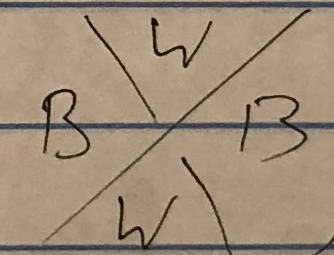
\includegraphics[width=0.5\textwidth]{crossing_coloring.png}
\caption{Black and white coloring of a crossing.}
\label{fig:bw_coloring}
\end{figure}
\item Given a Kauffman state $S$, 
\begin{align}
M\left( S \right) &= A\left( S \right) + \frac{\# \text{positive crossings} - 
\# \text{black regions}+1}{2}\\
A\left( S \right) &= M\left( S \right) - \frac{\sigma\left( K \right)}{2}
\end{align}
\item For an alternating knot, 
\begin{equation}
\sigma\left( K \right) = \# \text{Black regions} -  \# \text{Pos} - 1
\end{equation}
This exercise gives us the Knot Floer homology for an alternating knot.
\item This part deals with a simplified version of the Kauffman clock transform.
This transform can be visualized in \cref{fig:clock_transform_simple}.
\begin{figure}
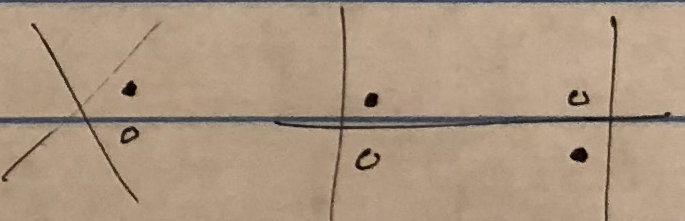
\includegraphics[width=0.5\textwidth]{clock_transform.png}
\caption{The simplified clock transform of a Kauffman state.}
\label{fig:clock_transform_simple}
\end{figure}
Prove the following:
\begin{thm}
Any two Kauffman states can be connected by a clock transform.
\end{thm}
\end{enumerate}
\end{exr}

\begin{prop}
The number of positive crossings does not depend on the orientation of the knot.
\end{prop}

\begin{rmk}
The signature of a knot was originally defined to be the signature of $A + A^T$ where
$A$ is the Seifert form.
\end{rmk}

\begin{prop}
The Alexander polynomial of an alternating knot is also alternating.
\end{prop}

So we have seen the unknotting number and the Seifert genus as invariants of a knot, but
there is also the smooth $4$-ball genus $g_4\left( K \right)$. 
Given a knot $K$, $g_4\left( K \right)$ is the minimal genus of a smoothly embedded surface in $D^4$
with $K$ as the boundary. 
There is a topological version of this, where we require a locally flat embedding.

There is a special case of this.
A knot $K$ is called smoothly sliced if $g_4\left( K \right) = 0$.

\begin{exr}
\begin{enumerate}
\item
Show that
\begin{equation}
g_4\left( K \right) \leq u\left( K \right)
\end{equation}
\item
Consider the right- and left-handed trefoil, 
and consider their connected sum as in \cref{fig:trefoil_sum}.
Prove that $g_4 = 0$.
\begin{figure}
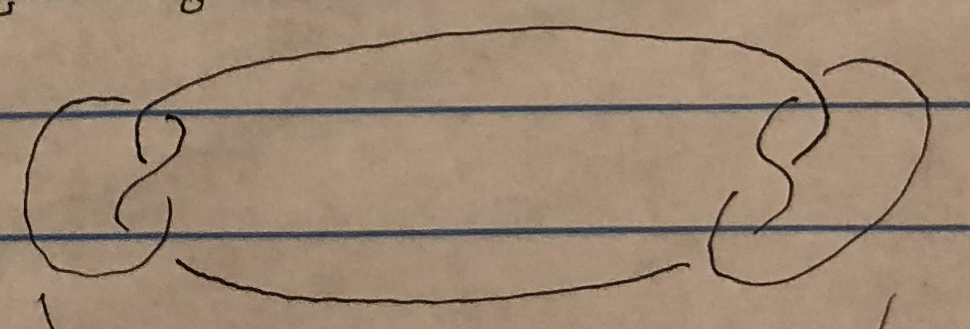
\includegraphics[width=0.5\textwidth]{sum_trefoil.png}
\caption{The connected sum of the right and left-handed trefoil.}
\label{fig:trefoil_sum}
\end{figure}
\item Show that the unknotting number of the connected sum of the two trefoil 
knots has unknotting number $2$.
\item The Conway knot and Kinoshita-Terasaka knots are in \cref{fig:conway_kino}.
The Conway knot has $g = 3$, and the Kinoshita-Terasaka knot has $g =2$.
\begin{figure}
\centering
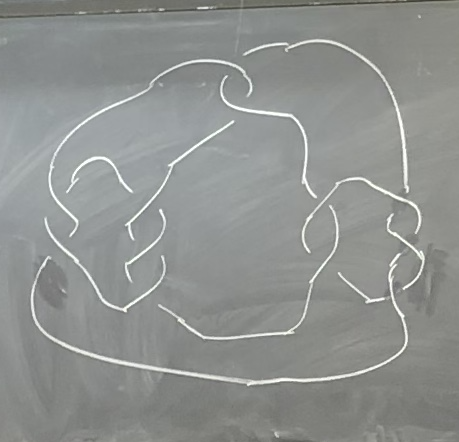
\includegraphics[width=0.4\textwidth]{conway_knot.png}
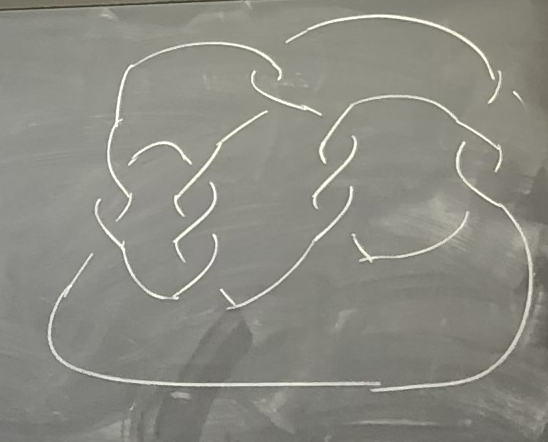
\includegraphics[width=0.4\textwidth]{kino_knot.png}
\caption{The Conway knot and Kinoshita-Terasaka knot.}
\label{fig:conway_kino}
\end{figure}
Show that $g_4 = 0$ for the Kinoshita-Terasaka knot.
There is a conjecture:
\begin{con}
$g_4 \neq 0$
\end{con}

\item Suppose we want to study $4$-manifolds.
So if a compact smooth $4$-manifold is homeomorphic to $S^4$, is it diffeomorphic?
That is, is there an exotic $S^4$? The smooth Poincar\'e conjecture suggests no.
There is an idea that goes as follows. 
Consider some $\Sigma^4$ which is potentially exotic.
Look at $S^4$, and consider a generic point. 
Then view $S^3$ as a neighborhood of this point. 
Consider some knot $K$ in a neighborhood in both of these manifolds, 
and ask what the $g_4$ is for the knot in $S^4$. 
Then consider the analogous $g_\Sigma$ in $\Sigma^4$. 
If we find any such knot for which these numbers are different, then $\Sigma$ must be exotic. 
So the hope is to find a $\Sigma$ and a knot $K$ for which $g_4 \neq g_\Sigma$. 

Show that $g_\Sigma\left( K \right) \leq g_4\left( K \right)$.
\end{enumerate}
\end{exr}

As it turns out, we always have the inequality $\abs{S\left( K \right)/2} \leq g_4$, 
but we actually have that this is bounded by $g_\Sigma$ as well.
Similarly
\begin{align}
\abs{\tau} \leq g_4
&&
\abs{\tau} \leq g_\Sigma
\end{align}

The fact that knot Floer homology detects the Seifert genus leads to the following:

\begin{cor}
$\hatt{\HFK}\left( K \right)$ has dimension one iff $K$ is the unknot.
\end{cor}

\section{Bordered knot Floer homology}

In the previous section we met an invariant $\CFK\left( K \right)$ of a knot $K$.
We now meet a way to calculate this, using bordered techniques.
The generic idea, will be to slice the knot projection up into a finite number of pieces, where
each slice crosses the projection $2n$ times. Then we can associate a special sort of algebra
to these $2n$ crossings, and then associate some sort of (bi)module over this algebra to each slice.
Then we can pair these objects with each other, and sort of scan through the knot
to calculate $\CFK\left( K \right)$.

\subsection{Upper Kauffman states}

An \emph{upper diagram} is some slice of the knot as in \cref{fig:upper_diagram}.
The \emph{bridge number} $n$ is the number of ``arcs'' above the line cutting the knot.
Equivalently, there are $2n$ intersection points of the knot with this line.\footnote{
Since there are finite intersection points, we can set this up so that the line
only goes through edges and not crossings or the ``top'' of a loop, so the generic 
upper diagram does indeed have $2n$ intersections.}

\begin{figure}
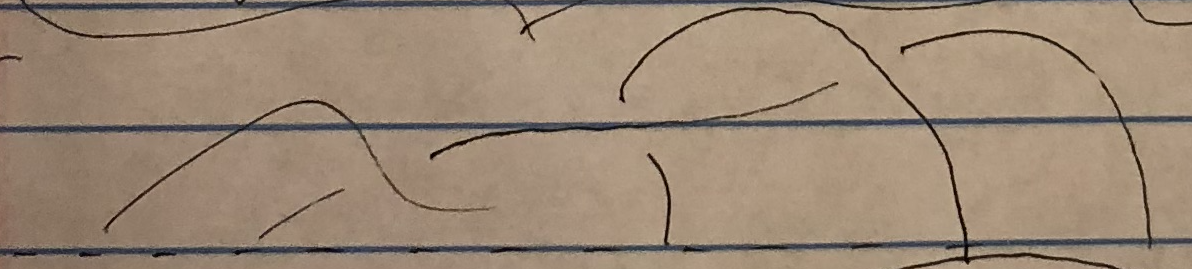
\includegraphics[width=0.5\textwidth]{upper_diagram.png}
\caption{An upper diagram for some knot $K$.}
\label{fig:upper_diagram}
\end{figure}

A \emph{local state} will be the collection of $n$ integers $x_1 , \cdots , x_n$
which satisfy $1 \leq x_1 < \cdots < x_n \leq 2n-1$.
Then an upper Kauffman state is a collection of $k$ corners $\left( c_1 , \cdots , c_k \right)$
and a local state $x_1 , \cdots , x_n$ such that every region either has a unique corner, 
or a unique marking on its boundary.
Some examples are shown in \cref{fig:upper_kauffman_state,fig:local_states}

\begin{figure}
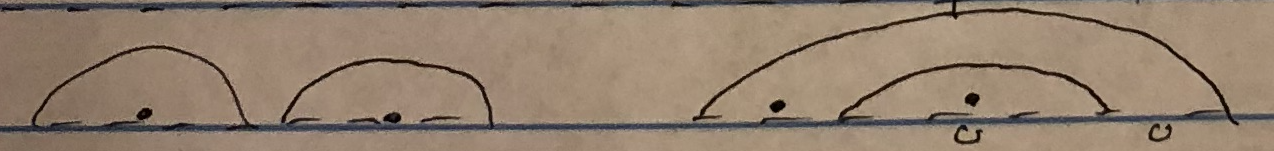
\includegraphics[width=0.5\textwidth]{upper_states1.png}
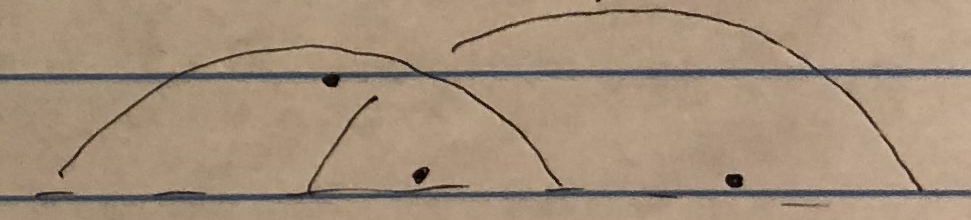
\includegraphics[width=0.5\textwidth]{upper_states2.png}
\caption{Examples of upper Kauffman states.}
\label{fig:upper_kauffman_state}
\end{figure}

\begin{figure}
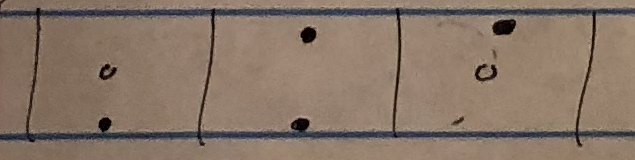
\includegraphics[width=0.5\textwidth]{local_states.png}
\caption{The three local states corresponding to $n = 2$.}
\label{fig:local_states}
\end{figure}

Note that if we are willing to take these local markings as the marked edges for the loops
below the cut, then these are actually honest Kauffman states.


\subsection{Construction of the algebra $\cC\left( n \right)$}

We want to associate some sort of bimodule to each slice of our knot
projection. In order to do this, we first need to define the algebra $\cC\left( n \right)$
over which our bimodules will be generated.
$\cC\left( n \right)$ will be the quotient of a larger algebra $\cC_0\left( n \right)$ which we
now define.

The object $\cC_0\left( n \right)$ will be a graded algebra over
$\FF\left( U_1 , \cdots , U_{2n} \right)$.
The basic idempotent elements $I_x$ 
of $\cC_0\left( n \right)$ will correspond to local states $x$, and 
will generate an idempotent ring $I\left( n \right) \sub \cC_0\left( n \right)$
given by the relations:
\begin{equation}
I_x \cdot I_y = 
\begin{cases}
I_x & x = y \\
0 & x\neq y
\end{cases}
\end{equation}
The unital element will be
\begin{equation}
1 = \sum_{x\in \text{ local states }} I_x
\end{equation}

This algebra $\cC_0\left( n \right)$ is almost a polynomial ring.
In particular, we have the following identification of 
$\FF\left[ U_1 , \cdots , U_{2n} \right]$-modules:
\begin{equation}
I_x \cC_0\left( n \right) I_y
\simeqq \FF\left[ U_1 , \cdots , U_{2n} \right]
\end{equation}
We will also define a multiplication:
\begin{equation}
\left( I_x \cC_0\left( n \right) I_y\right) * 
\left( I_y \cC_0\left( n \right) I_z \right)
\fromto
I_x \cC_0\left( n \right) I_z
\end{equation}

Given a local state $x$, we define the weight-vector $v^x\in \ZZ^{2n}$, by 
\begin{equation}
v^x_i = \# \left\{ x_j \in x \st x_j \geq i\right\}
\end{equation}
Then for two states $x , y$ we define the minimal relative weight 
$r^{x,y}\in \left( 1/2 \ZZ \right)^{2n}$ by
\begin{equation}
r^{xy}_i = \abs{v_i^x - v_i^y}
\end{equation}
This $i$th component of this minimal relative weight 
returns the number of crossings of the $i$th strand between $x$ and $y$.

\begin{exm}
Take $n = 4$.
In this case $v\left( x , y \right) \in \ZZ^{4}$
As we can see in \cref{fig:weight_2}, 
we get $r^{xy} = \left( 0,1,1,0 \right)$.
\begin{figure}
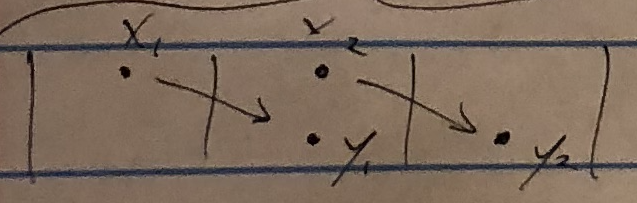
\includegraphics[width=0.5\textwidth]{weight_2.png}
\caption{$r^{xy}$ for $n = 2$.}
\label{fig:weight_2}
\end{figure}
\end{exm}

Now recall the identification of $I_x \cC_0\left( n \right) I_y$ with the polynomial ring
over $U_1 , \cdots , U_{2n}$. 
Write this identification as:
\begin{equation}
a\left( x , y , \cdot \right):
\FF\left[ U_1 , \cdots , U_{2n} \right] \fromto
I_x \cC_0\left( n \right) I_y
\end{equation}
For any monomial $p\in \FF\left[ U_1 , \cdots , U_{2n} \right]$ we can write
$p = U_1^{t_1} \cdots U_{2n}^{t_{2n}}$ for some $t_1 , \cdots , t_{2n}$.
Now a grading is specified by the \emph{weight}:
\begin{equation}
w\left( a\left( x , y , p \right) \right) = 
r^{xy} + \left( t_1 , \cdots , t_{2n} \right)
\end{equation}

We now define the multiplication mentioned above by the relations:
\begin{equation}
\begin{cases}
a\left( x , y , p_1 \right) * a\left( s , r , p_2 \right) = 0
& y\neq s \\
a\left( x , y , p_1 \right) * a\left( s , r , p_2 \right) = 
a\left( x , r, p_3 \right)
& y = s
\end{cases}
\end{equation}
where $p_3$ is such that $w$ is additive.
We can write this out explicitly as follows. 
Consider three states $x$, $y$, and $z$. 
Then we will write $p_3$ such that
\begin{equation}
a\left( x , y , p_1 \right) * a\left( y , z , p_2 \right) = 
a\left( x , r, p_3 \right)
\end{equation}
If we define $t_i = w_i^{xy} + w_i^{yz} - w_i^{xz}$ for $i\in \left\{ 1 , \cdots , 2n \right\}$,
then we can write $p_3$ as
\begin{equation}
p_3 = U_1^{t_1}\cdots U_{2n}^{t_{2n}} p_1 p_2
\end{equation}

\begin{exm}
$a\left( x , x , 1 \right)$ gives us the idempotent $I_x$.
Also, $a\left( x , y , 1 \right) a\left( u , r , 1 \right) = a\left( x , y , U_2 \right)$.
\end{exm}

\begin{exm}
Let's consider $x = \left\{ 1,2 \right\}$ and look at $\cC\left( n \right)$. 
Then $a\left( x , x , U_4 \right) = 0$.
We also have 
\begin{equation}
a\left( x , x , U_1U_2U_3\right) = 
a\left( x,y,1 \right) \ubr{a\left( y , y , U_1 \right)}{=0} a\left( y,x,1 \right) = 0
\end{equation}
\end{exm}

Now what are the generators of $\cC_0\left( n \right)$ 
over the idempotent ring $I\left( n \right)$?
Equivalently, what do we need besides the elements $I_x$ to generate $\cC_0\left( n \right)$
over $\FF$?
First we can define the elements:
\begin{equation}
U_i \ceqq \sum_{x} a\left( x , x , U_i \right)
\end{equation}
Now let $x$ be some state containing $j-1$ and not $j$. 
Then we form a new state by define $y = \left( x\un j \right) \minus \left\{ j-1 \right\}$. 
So we have a dot in $j$ instead of $j-1$.
Then we define:
\begin{equation}
R_i \ceqq \sum_{x\st j-1\in x, j\not \in x} a\left( x , y , 1 \right)
\end{equation}
Note that we have:
\begin{equation}
I_x R_j = 
\begin{cases}
a\left( x , y , 1 \right)
& j-1\in x , j\not \in x \\
0 & \text{ otherwise }
\end{cases}
\end{equation}
Similarly we define
\begin{equation}
L_j \ceqq 
\sum_{y\st j\in y , j-1 \not \in y }
a\left( y , x , 1 \right)
\end{equation}

\begin{rmk}
$L_j$ and $R_j$ correspond to shifting left and right respectively.
\end{rmk}

\begin{wrn}
It is not always the case that acting $L$ and $R$ gives us $U$.
For example $a\left( x , x , 1 \right) U_i$ is not $L_i R_i$ and not
$R_i L_i$.
\end{wrn}

Now we want to show $\cC_0\left( n \right)$ is itself graded by $w$:

\begin{prop}
The grading, $w$, on $I_x \cC_0\left( n \right) I_y$, 
descends to $\cC_0\left( n \right)$ itself.
\end{prop}

\begin{proof}
We just have to show:
\begin{equation}
w\left( a\left( x , y , 1 \right) * a\left( y , z , 1 \right) \right) = 
w\left( a\left( x , y , 1 \right)  \right) + 
w\left( a\left( y , z , 1 \right) \right)
\end{equation}
but the definition of $p_3$ was rigged for this to be the case.
\end{proof}

In light of this proposition, we will now write the multiplication $*$
without the symbol.

\begin{prop}
The algebra $\cC_0\left( n \right)$ is generated over $\FF$ by $L_i$, $R_i$, $U_i$, 
and $I_x$.
\end{prop}

Now we still need to define $\cC\left( n \right)$ itself.
As promised we will quotient out by an ideal.
In particular, we generate a two-sided ideal $J$ by the following:
\begin{align}
L_{i+1} L_i &&
R_i R_{i+1} 
\end{align}
and if $\left\{ x_1 , \cdots , x_k \right\} \cap \left\{ j-1 , j \right\} = \emp$, 
then
\begin{equation}
I_x U_j
\end{equation}
Then, finally, 
\begin{equation}
\cC\left( n \right) \ceqq 
\cC_0\left( n \right) / J
\end{equation}

We can write this different ways. 
For example, we want $a\left( x , x, u_i \right)$ to be in the ideal whenever $i \not \in x$ 
and $i -1 \not \in x$ is equivalent to the third condition above.

The interpretation here 
is that the elements of $\cC\left( n \right)$ should not be able
to move coordinates in the idempotent states by more than one unit.

\begin{exm}
For $n = 1$, we have
\begin{align}
I\left( 1 \right) = \FF&&
\cC\left( 1 \right) = \FF\left[ u_1 , u_2 \right] /
\left\{ u_1 \cdot u_2 = 0 \right\}
\end{align}
In the end we will get a chain complex over $\cC\left( 1 \right)$.
We can view this as a chain complex over $\FF$ by the forgetful map
bringing $u_1$ and $u_2$ to $0$ in $\FF$.
This gives us the simplest version of knot Floer homology. 
We could alternatively map $\cC\left( 1 \right)$ to $\FF\left[ u_1 \right]$ by mapping $u_2 \mapsto 0$.
This gives a filtrated complex, 
by allowing for differentials that decrease the Alexander grading
and not the Maslov grading. The total homology is an invariant, 
but it is the same for every knot, 
in particular it gives $\FF$.
We do however get an interesting integer valued invariant called $\tau\left( K \right)$.
\end{exm}

\begin{exr}
Take $n = 3$, and $x = \left\{ 2,3,5 \right\}$ and $y = \left\{ 1,3,5 \right\}$. 
Now take $I_x J I_y \subeq I_x \cC_0 I_y$.
Let's view $I_x \cC_0 I_y$ as a polynomial algebra $\FF\left[ u_1 , \cdots , u_{2n} \right]$. 
So there is a new object
\begin{equation}
J_{x,y} \subeq \FF \left[ u_1 , \cdots , u_{2n} \right]
\end{equation}
Show that this is an ideal inside the polynomial algebra in the usual sense, 
and find generators of this ideal.
\end{exr}

\begin{exr}
Suppose we have the two local states in \cref{fig:exr_states}
\begin{figure}
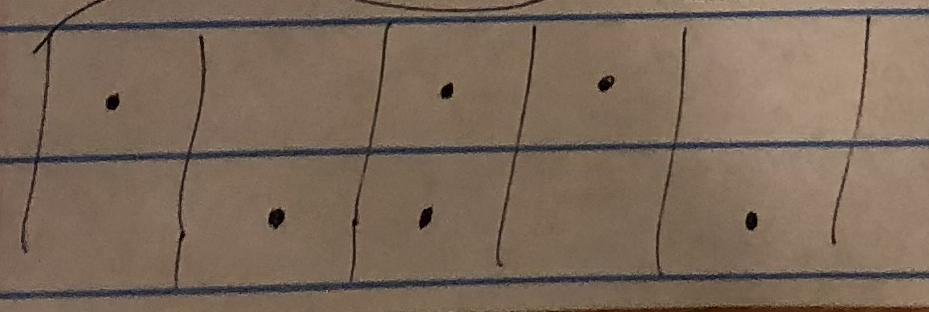
\includegraphics[width=0.5\textwidth]{2_local_states.png}
\caption{Two local states of the upper diagram of a knot.}
\label{fig:exr_states}
\end{figure}
Show that $a\left( x , y , u_3u_4 \right) \in J$.
\end{exr}

\subsection{$D$-structure associated with an upper diagram}

For any slice of a knot at time $t$, we can consider the upper diagram as in the preceding subsection.
We can then consider all of the possible upper Kauffman states of this upper diagram.
Write $\DFK$ for the $\FF$-vector space generated by the upper Kauffman states.
We will turn this into a curved $D$-structure\footnote{See \cref{app:d_structures} 
for the definition of a (curved) $D$-structure.}
by defining a structure map $\dd^1: \DFK \fromto \cC\left( n \right) \tp \DFK$.
Explicitly this will be defined by counting pseudo-holomorphic disks:
\begin{equation}
\dd \mathbf{x} = \sum_y\sum_{B\in \pi_2\left( \mathbf{x} , \mathbf{y} \right),\mu\left( B \right) = 1}
\#\left(\frac{\cM^B\left( \mathbf{x} , \mathbf{y} \right) }{\RR}\right)\cdot c\left( B \right) \tp y
\end{equation}

\subsection{$DA$-bimodule associated with a crossing}

See \cref{app:da_bimodules} for the definition of a $DA$-bimodule.

\subsection{$A$-structure associated with a lower diagram}

See \cref{app:d_structures} for the definition of an $A$-structure.

\appendix
\section{$D$-structures and $\cA_\infty$ modules}
\label{app:d_structures}

Let $\cA$ denote a dg algebra\footnote{
That is, a graded vector space equipped with a differential and associative multiplication
compatible by the Leibniz rule.}

A (right) $\cA_\infty$-module over $\cA$ is a $\ZZ$-graded
$\FF$-module $M$ together with degree $0$, $\FF$-linear maps
\begin{equation}
m_{j + 1}: M\tp \cA^{\tp j} \fromto M
\end{equation}
for $j\in \NN$ such that for each $i$, $x\in M$, and 
$a_1 , \cdots , a_i\in A$, 
\begin{multline}
0 = \sum_{j = 0}^{i-1}
m_{i - j} \left( m_{ j+1}\left( x , a_1 , \cdots , a_n \right) , 
a_{j + 1} , \cdots , a_i \right) \\
+ \sum_{j = 1}^i \sum_{k = 1}^{i - j + 1} m_{i - j + 1}
\left( x , a_1 , \cdots , a_{k-1} , \mu_j\left( a_k , \cdots , a_{k+j} \right),
a_{k + j + 1} , \cdots , a_i\right)
\end{multline}

These relations are known as the $\cA_\infty$ relations, and
can be understood as follows.
Consider trees which have $k$ inputs and a single output, where the furthest
left input is privileged.
Then each tree $T$ represents a map $m\left( T \right):\cA^{\tp k} \fromto \cA$.
The operation of a vertex of valence $n$ is labelled by $m_n$.
An example is shown in \cref{fig:trees}.

\begin{figure}
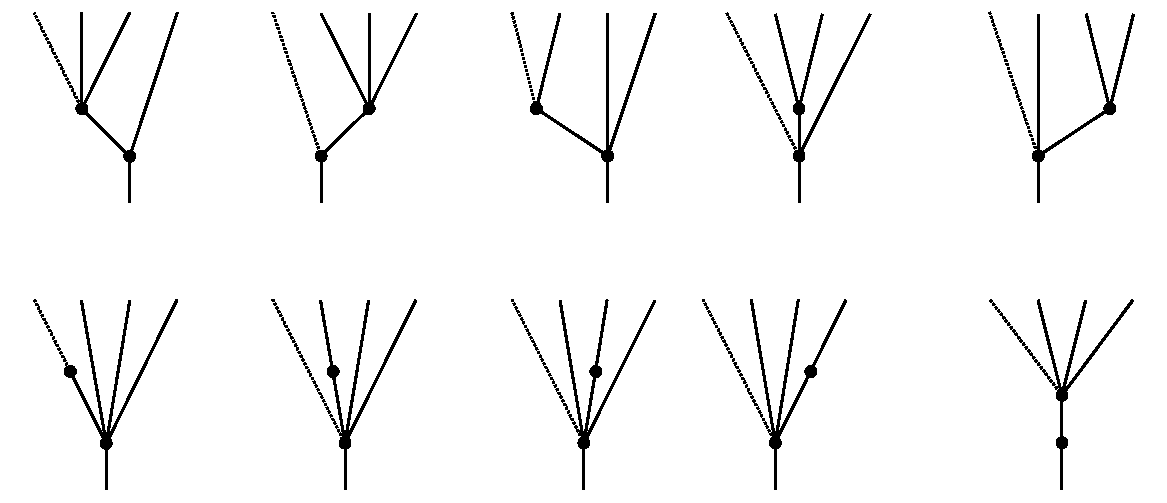
\includegraphics[width=0.7\textwidth]{trees.pdf}
\caption{The sum of the operations associated to these trees vanishes; 
for example, the tree on the top right contributes
$m_3\left( x,a,m_2\left( b,c \right) \right)$.}
\label{fig:trees}
\end{figure}

A type $D$-structure over $\cA$ is a graded vector space $X$, 
equipped with the map
\begin{equation}
\dd^1: X\fromto \cA \tp X
\end{equation}
satisfying the structure equation:
\begin{equation}
\left( \mu_2 \tp \id_X \right) \comp 
\left( \dd^1 \tp \id_X \right) \comp \dd^1
+ \left( \mu_1 \tp \id_X \right) \comp \dd^1 = 0
\end{equation}

Now we can iterate this map to get
\begin{equation}
\dd^j : X\fromto \cA^{\tp j} \tp X
\end{equation}
defined inductively by
\begin{equation}
\dd^j \ceqq
\left( \id_{A^{\tp \left( j-1 \right)} }\tp \dd^1 \right)\comp
\dd^{j-1}
\end{equation}

\section{$DA$-bimodules}
\label{app:da_bimodules}

\todo{clean}

\begin{defn}
Let $\cA$ and $\cB$
be $\cA_\infty$-algebras over $\FF$.
Then a type $DA$ bimodule $^{\cA} N_\cB$ over $\cA$ and 
$\cB$ consists of a graded $\left( \FF, \FF \right)$-bimodule $N$
and degree $0$, $\left( \FF , \FF \right)$-linear maps
\begin{equation}
\dd_{1 + j}^1: N\tp B^{\tp j} \fromto A \tp N
\end{equation}
which satisfy the following compatibility condition.
Let $\dd^1 = \sum_j \dd^1_j$, and define
\begin{equation}
\dd^i:N\tp T^*\left( B \right) \fromto
A^{\tp i} \tp N
\end{equation}
by $\dd^0 = \id$, and 
\begin{equation}
\dd^{i+1} = \left( \id_{A^{\tp i}} \tp \dd^1 \right) \comp 
\left( \dd^i \tp \id_{T^* B} \right)\comp
\left( \id_N \tp \Delta \right)
\end{equation}
where $\Delta : T^*\left( B \right)\fromto T^*\left( B \right)\tp T^*\left( B \right)$
is the canonical comultiplication. 
Now define
\begin{equation}
\dd^N : N\tp T^*\left( B \right) \fromto \barr{T^*}\left( A \right)\tp N
\end{equation}
by 
\begin{equation}
\dd^N = \sum_{i = 0}^\infty \dd^i
\end{equation}
Then we must have:
\begin{equation}
\dd^N \comp \left( \id_N \tp \barr{D}^\cB\right) +
\left( \barr{D}^\cA \tp \id_N \right)\comp \dd^N = 0
\end{equation}
We will write the category of such bimodules as
$^{\cA}\Mod_\cB$.
\end{defn}

This should be thought of as something which is simultaneously a 
$D$-structure and an $\cA_\infty$-algebra.

\section{Box tensor product}

\todo{clean}

There is a natural pairing between $\cA_\infty$ modules $M$
and $D$-structures $X$ over $\cA$. In particular, we can
equip the vector space $M\tp X$ with the endomorphism
\begin{equation}
D\left( p\tp x \right) = 
\sum_{j = 0}^\infty
\left( m_{j+1} \tp \id_X \right)\comp \dd^j\left( x \right)
\end{equation}
Note that this might not be a finite sum. 
The module $M$ is said to be \emph{algebraically bounded} if
$m_j = 0$ for $j$ sufficiently large.

\todo{combine these definitions}

\begin{defn}
For $\cA$ an $\cA_\infty$-algebra, $\amod{M}{\cA} \in \aMod{\cA}$, 
and $\dmod{N}{\cA}\in \dMod{\cA}$, with at least one of $\amod{M}{\cA}$ or $\amod{N}{\cA}$
bounded, define $\amod{M}{\cA} \boxtp \dmod{N}{\cA}$ 
to be a chain complex with underlying space
$M\tp_k N$ and boundary operator
\begin{equation}
\p \ceqq \left( m_M \tp \id_N \right)\comp \left( \id_M \tp \dd^N \right)
\end{equation}
\end{defn}

So we have seen how to get a $D$-structure from the box-tensor
product of a $D$-structure and an $\cA_\infty$ module. 
Now we need an analogous pairing between $DA$-bimodules. 
Roughly speaking, the construction forgets the $A_\infty$ structure on one,
and forgets the $D$-structure on the other, and then just using the construction
from above on these simpler objects. 

More formally, consider the forgetful functors:
\begin{equation}
\begin{tikzcd}
\DAMod{\cA}{\cB} \arrow{r}{\cF}& \aMod{\cB}\\
\DAMod{\cA}{\cB} \arrow{r}{\cF}& \dMod{\cA}
\end{tikzcd}
\end{equation}
Then we can define the following:
\begin{defn}
Let $\damod{M}{\cA}{\cB} \in \DAMod{\cA}{\cB}$ and
$\damod{N}{\cB}{\cC}\in \DAMod{\cB}{\cC}$.
Then define the box-tensor product of these to be:
\begin{equation}
\damod{M}{\cA}{\cB} \boxtp \damod{N}{\cA}{\cB} \ceqq
\cF\left( \damod{M}{\cA}{\cB} \right)_\cB \boxtp
^{\cB}\cF\left( \damod{N}{\cB}{\cC} \right)
\end{equation}
with $DA$ structure given by
\begin{equation}
\dd_j^{M\boxtp N} \ceqq
\sum_n
\id_M \tp \dd_{1 + j}^N \comp \id_N \tp \dd_{1 + j}^M
\end{equation}
\end{defn}

So the composition $\dd_j^{M\boxtp N}$ maps:
\begin{equation}
M\tp N \tp A^{\tp j} \fromto B^{\tp k} \tp M \tp N \fromto
C\tp M \tp N
\end{equation}

\end{document}
